\chapter{Methodology on Vision-Based Defect Detection System for Industrial Quality Inspection}
\label{ch:method}

This chapter outlines the complete, reproducible engineering methodology of the proposed automated robotic vision inspection system. The framework integrates an industrial optomechanical imaging station, an exhaustive 5,065-image flaw dataset, an optimized single-stage YOLOv8 Oriented Bounding Box (YOLOv8-OBB) neural network, mathematically rigorous multi-task loss formulations, micro-defect augmentation suppression techniques, and real-time edge acceleration via ONNX Runtime, TensorRT, and ROS2-PLC industrial middleware. Each subsystem is systematically formulated, derived, and explained below.

%------------------------------------------------------------------
\section{Proposed Robotic Vision System Architecture}
\label{sec:architecture}

The automated inspection system operates as an inline, deterministic edge inspection station positioned directly downstream of the high-speed container thermoforming and cooling stages. The inspection station comprises an optomechanical enclosure, an optical imaging payload, an edge computing industrial node, a high-speed conveyor belt, and a downstream pneumatic solenoid rejection mechanism.

To mitigate ambient factory illumination variance and eliminate intense specular glares on curved polymer surfaces, the imaging station utilizes an opaque optomechanical enclosure. Illumination is provided by a dual-wavelength coaxial diffuse ring LED illuminator (5200K daylight white balanced with low-angle diffuse red backlighting), providing uniform photometric radiance across both the horizontal container flange and the concave thermoformed bowl.

Image acquisition is performed by a 5.0-megapixel industrial CMOS area-scan camera (Basler ace2, Sony IMX547 sensor, global shutter) paired with a high-precision bilateral telecentric lens (0.24$\times$ magnification, working distance 180~mm). Telecentric optics eliminate perspective distortion and maintain a constant magnification ratio across varying casing heights on the conveyor. An optical retroreflective photoelectric sensor detects the leading edge of oncoming casings, triggering camera hardware exposure with sub-microsecond synchronization.

Figure~\ref{fig:sys_pipe} illustrates the complete hardware-software block diagram of the automated robotic vision defect detection, edge inference, and high-speed pneumatic ejection pipeline.

\begin{figure}[htbp]
\centering
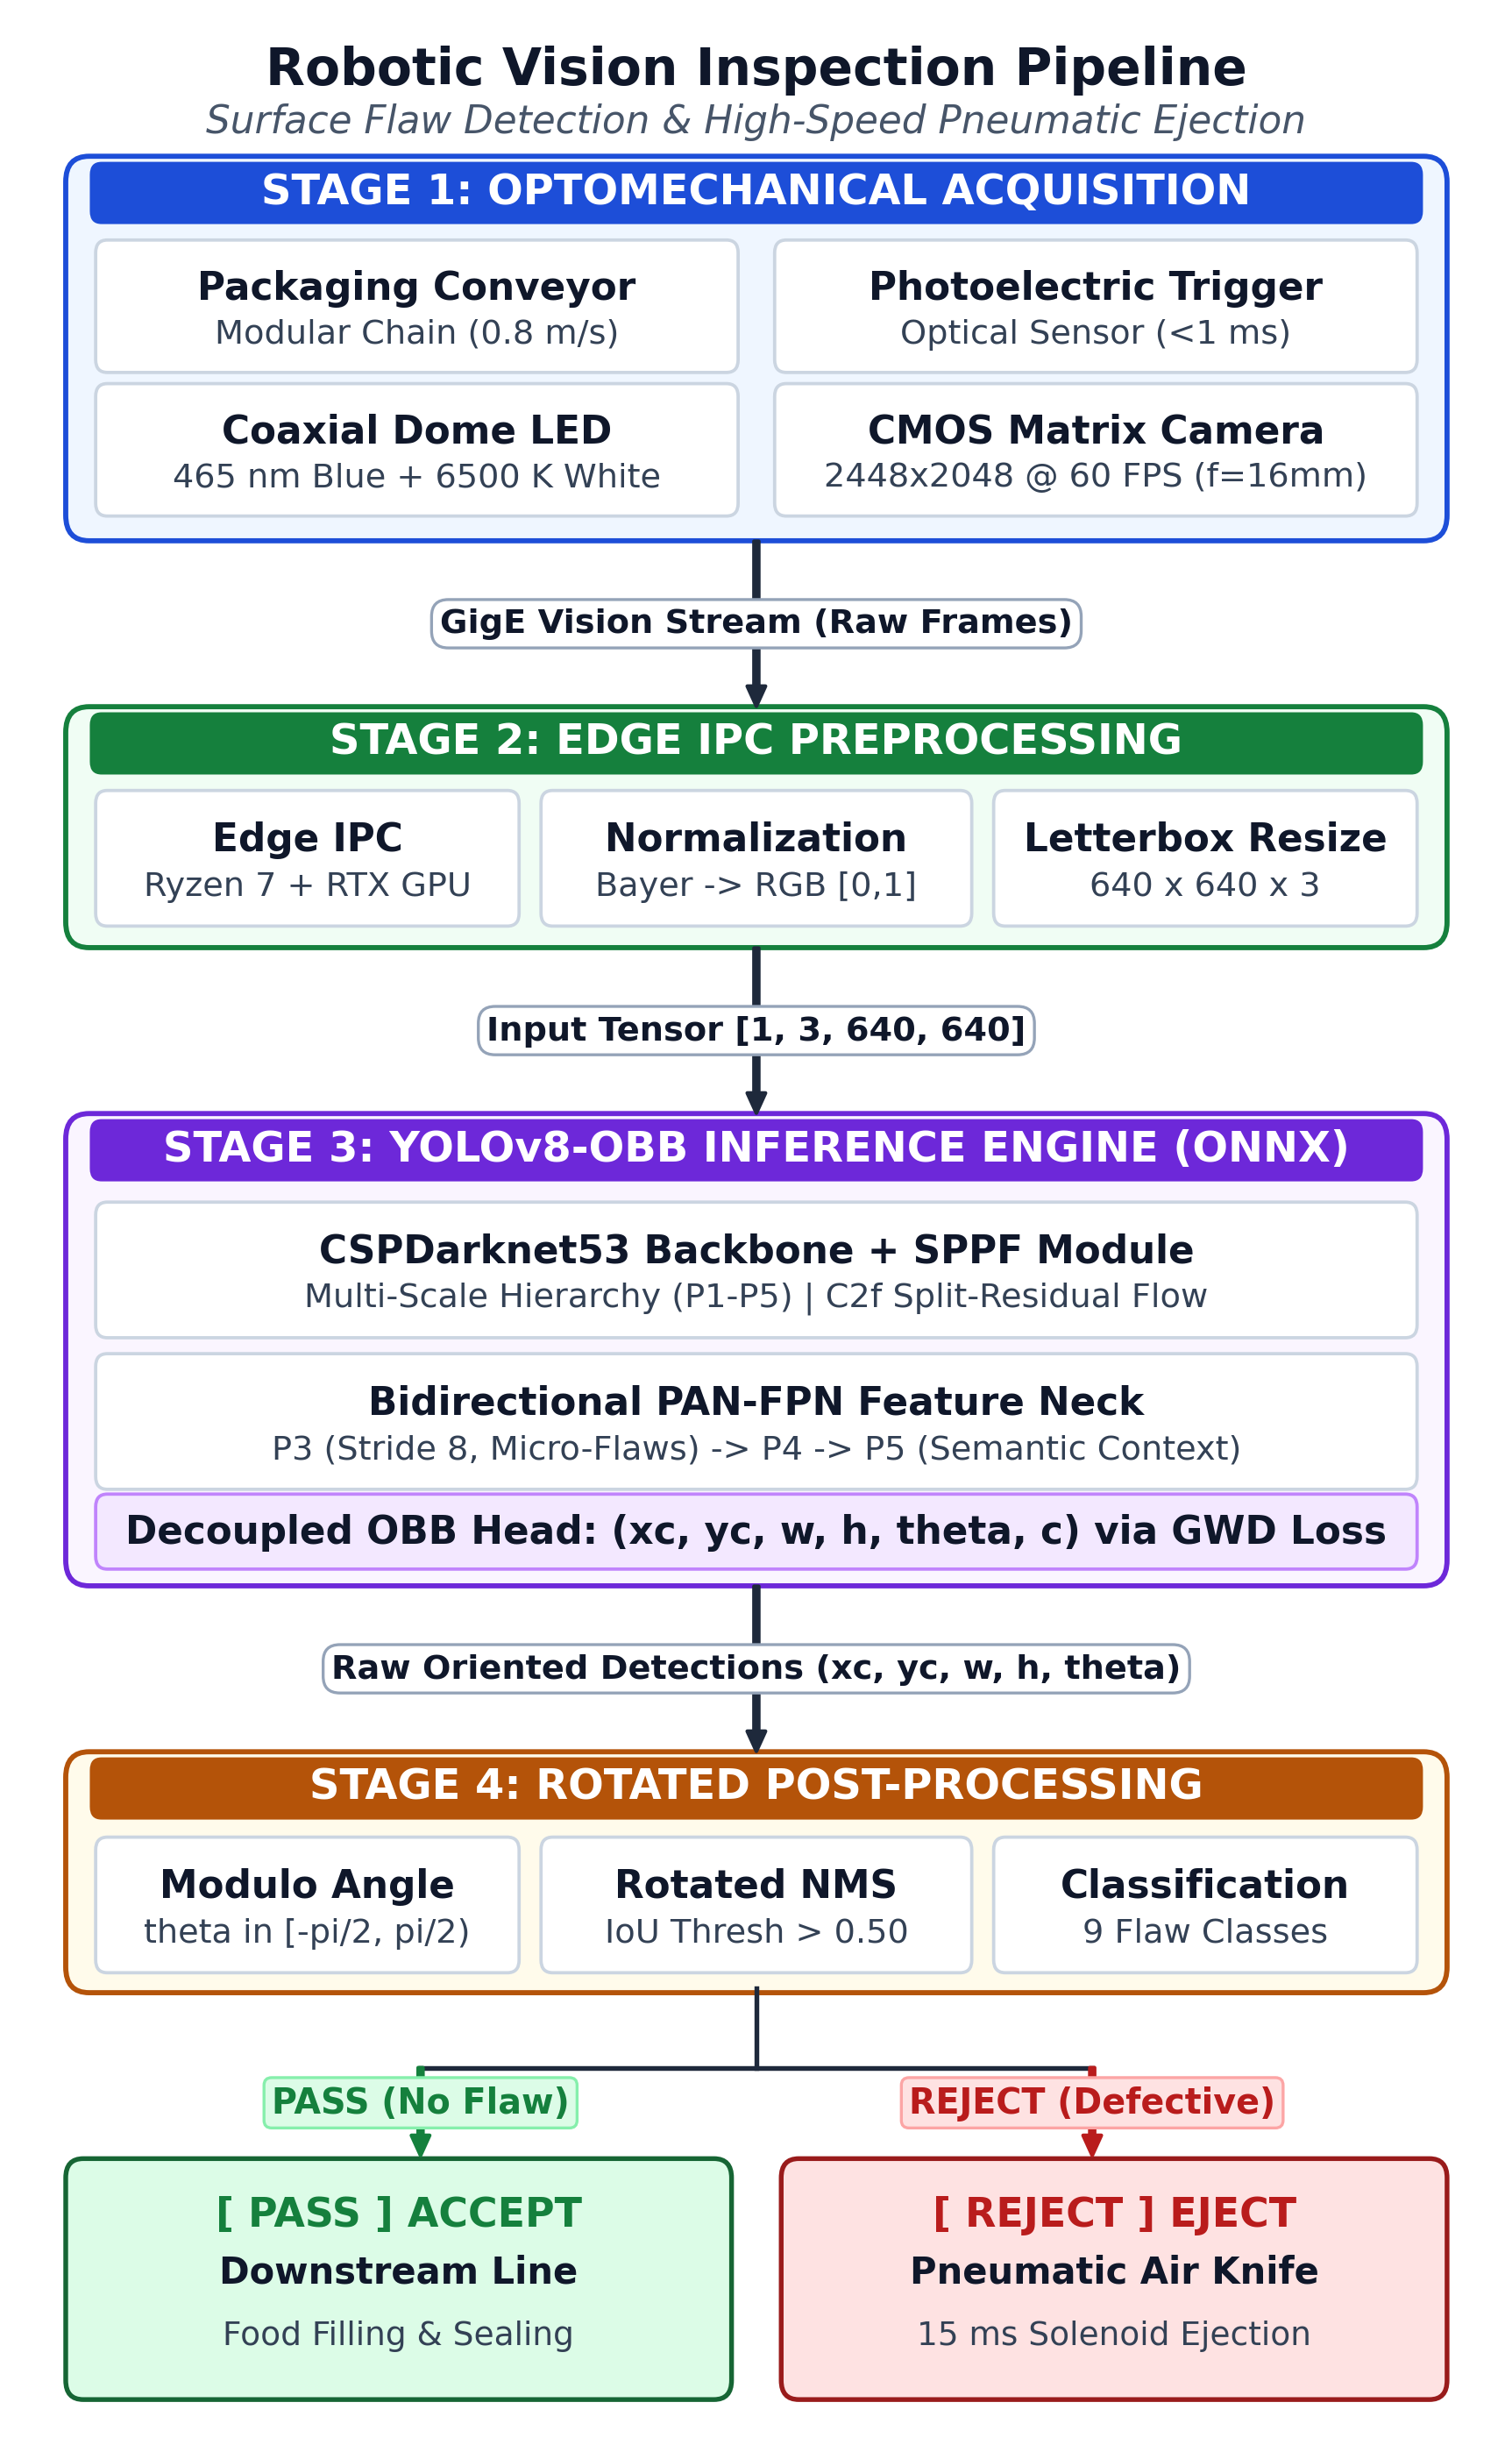
\includegraphics[width=0.95\textwidth]{images/system_pipeline.png}
\caption{Architectural block diagram of the automated robotic vision defect detection, edge inference, and high-speed pneumatic ejection pipeline}
\label{fig:sys_pipe}
\end{figure}

To illustrate the physical implementation of this robotic inspection cell, Figure~\ref{fig:factory_enclosure} displays multiple photographic perspectives of the operational industrial packaging conveyor line deployed within the cleanroom production environment. The optomechanical inspection station is housed inside a sanitary stainless steel (SUS304) enclosure that straddles the modular conveyor line. The workstation is equipped with an articulated swing-arm assembly carrying an industrial touchscreen Human-Machine Interface (HMI) terminal, an auxiliary operational monitor, overhead pneumatic maintenance service lines, and a multi-tiered tri-color signal tower light that provides instantaneous visual status warnings to production supervisors upon detecting severe defect bursts.

\begin{figure}[htbp]
\centering
\includegraphics[width=0.88\textwidth]{images/factory_installation_enclosure.jpg}
\caption{Physical industrial packaging conveyor line and stainless steel optomechanical inspection cell enclosure}
\label{fig:factory_enclosure}
\end{figure}

%------------------------------------------------------------------
\section{Industrial Dataset Specification and Defect Taxonomy}
\label{sec:dataset}

Supervised training of high-fidelity oriented detectors requires a comprehensive, well-balanced industrial flaw dataset. An extensive benchmark dataset of 5,065 high-resolution ($640 \times 640$) images was acquired directly from production runs of thermoformed polypropylene (PP) rice meal packaging casings. The dataset captures genuine industrial defect variability across nine distinct flaw categories:

\begin{enumerate}
\item \textbf{Black Dots:} Minute carbonized polymer inclusions formed during barrel thermal degradation (mean dimensions $14 \times 14$~px).
\item \textbf{Defective Foreign Body:} Extraneous plastic shavings, fibrous threads, and mechanical debris embedded during trimming (mean dimensions $38 \times 16$~px).
\item \textbf{Flange Bad Cutting:} Ragged, torn, or non-uniform outer flange borders caused by misaligned trimming blades (mean dimensions $95 \times 18$~px).
\item \textbf{Insect:} Biological pest contaminants trapped on container surfaces (mean dimensions $42 \times 32$~px).
\item \textbf{Intense Scratch:} Deep mechanical gouges penetrating surface barrier layers, typically oriented obliquely (mean dimensions $115 \times 12$~px).
\item \textbf{Pinhole:} Sub-millimeter circular punctures ($<0.2$~mm) caused by trapped air bubbles during molding (mean dimensions $10 \times 10$~px).
\item \textbf{Scratch (Micro-abrasion):} Elongated, low-contrast superficial abrasions oriented diagonally across the casing floor (mean dimensions $82 \times 8$~px).
\item \textbf{Shrivel Wrinkle:} Material folding wrinkles and corrugations along curved sidewalls due to uneven thermoforming draw (mean dimensions $180 \times 24$~px).
\item \textbf{Yellow Point:} Thermal discolored polymer degradation patches caused by localized heater overheating (mean dimensions $22 \times 22$~px).
\end{enumerate}

Ground truth annotations were performed using oriented bounding boxes defined by five geometric parameters $[x, y, w, h, \theta]$, where $\theta$ denotes the rotation angle normalized in the range $[-\pi/2, +\pi/2]$. The dataset was partitioned into a training set of 4,674 images (22,610 defect instances) and an independent validation set of 391 images (1,867 defect instances). The comprehensive instance counts and geometric dimensional profiles are summarized in Table~\ref{tab:taxonomy}.

\begin{table}[htbp]
\centering
\small\singlespacing
\renewcommand{\arraystretch}{1.15}
\caption{Industrial Defect Taxonomy, Instance Distribution, and Geometric Dimensions Across Partitions}
\label{tab:taxonomy}
\begin{tabularx}{\textwidth}{|>{\raggedright\arraybackslash}X|>{\centering\arraybackslash}p{2.8cm}|>{\centering\arraybackslash}p{2.6cm}|>{\centering\arraybackslash}p{4.2cm}|}
\hline
\textbf{Defect Category} & \textbf{Train Instances} & \textbf{Val Instances} & \textbf{Mean Dimensional Area (px$^2$)}\\ \hline
Black Dots & 14,820 & 1,226 & $14 \times 14$\\ \hline
Defective Foreign Body & 1,050 & 87 & $38 \times 16$\\ \hline
Flange Bad Cutting & 290 & 23 & $95 \times 18$\\ \hline
Insect & 220 & 18 & $42 \times 32$\\ \hline
Intense Scratch & 360 & 29 & $115 \times 12$\\ \hline
Pinhole & 1,240 & 102 & $10 \times 10$\\ \hline
Scratch (Micro-abrasion) & 840 & 69 & $82 \times 8$\\ \hline
Shrivel Wrinkle & 3,180 & 263 & $180 \times 24$\\ \hline
Yellow Point & 610 & 50 & $22 \times 22$\\ \hline
\textbf{Total Instances} & \textbf{22,610} & \textbf{1,867} & --- \\ \hline
\textbf{Total Images} & \textbf{4,674} & \textbf{391} & --- \\ \hline
\end{tabularx}
\end{table}

%------------------------------------------------------------------
\section{YOLOv8-OBB Neural Network Architecture}
\label{sec:yolo_arch}

The proposed deep inspection model is based upon an optimized YOLOv8-OBB architecture. The network comprises three interconnected functional subsystems: a feature extraction Backbone, a multiscale Feature Pyramid Neck, and Decoupled Oriented Detection Heads.

\begin{itemize}
\item \textbf{Backbone Feature Extractor:} The backbone employs CSPDarknet enhanced with C2f (Cross-Stage Partial Bottleneck with two convolutions) modules. The C2f block splits high-resolution feature maps into gradient paths, combining low-level texture gradients with deep semantic features while maintaining gradient stability and low parameter count. A Spatial Pyramid Pooling -- Fast (SPPF) module pools features at receptive fields of $5 \times 5$, $9 \times 9$, and $13 \times 13$ to capture multi-scale context without increasing computational overhead.
\item \textbf{Multiscale PANet Neck:} The neck features an augmented Path Aggregation Network (PANet) combined with a Feature Pyramid Network (FPN). The bidirectional pathway aggregates rich spatial localization features from shallow layers ($P_3$, stride 8) with deep semantic representations from deep layers ($P_5$, stride 32). This multi-scale feature representation is essential for simultaneously localizing minute 10-pixel pinholes and extensive 180-pixel wrinkles.
\item \textbf{Decoupled Oriented Detection Heads:} Unlike standard YOLOv8, which couples classification and bounding regression into a single head, the YOLOv8-OBB architecture employs anchor-free decoupled detection heads. Three distinct convolutional branches independently predict: (i) class probability scores; (ii) bounding box center offsets and dimensions $[x, y, w, h]$; and (iii) the orientation rotation angle $\theta$. Decoupling the heads eliminates feature interference between classification gradients and angular regression updates.
\end{itemize}

%------------------------------------------------------------------
\section{Mathematical Derivations of Multi-Task Loss Formulation}
\label{sec:loss}

Training an oriented bounding box detector requires optimizing a multi-task composite loss objective that jointly penalizes classification errors, bounding box geometric misalignment, angular deviations, and boundary distribution uncertainties. The total loss $\mathcal{L}_{\text{total}}$ is formulated as:
\begin{equation}
\label{eq:total_loss}
\mathcal{L}_{\text{total}} = \lambda_{\text{cls}} \mathcal{L}_{\text{cls}} + \lambda_{\text{box}} \mathcal{L}_{\text{box}} + \lambda_{\text{dfl}} \mathcal{L}_{\text{dfl}} + \lambda_{\theta} \mathcal{L}_{\theta}
\end{equation}
where $\lambda_{\text{cls}} = 0.5$, $\lambda_{\text{box}} = 7.5$, $\lambda_{\text{dfl}} = 1.5$, and $\lambda_{\theta} = 2.5$ represent empirically calibrated loss balancing coefficients.

\subsection{Classification Loss: Varifocal Loss (VFL)}
\label{subsec:vfl}

Standard Focal Loss treats positive and negative samples symmetrically, weighting positive samples purely based on classification confidence. However, in high-precision defect inspection, candidate boxes with high IoU overlap must be prioritized. We employ Varifocal Loss (VFL), which incorporates the continuous IoU score $q$ between the predicted oriented box and the ground-truth box as the learning target for positive samples:
\begin{equation}
\label{eq:vfl}
\mathcal{L}_{\text{cls}} = \begin{cases} 
- q \left( q \log(p) + (1 - q) \log(1 - p) \right), & q > 0 \\ 
- \alpha p^{\gamma} \log(1 - p), & q = 0 
\end{cases}
\end{equation}
where $p \in [0, 1]$ denotes the predicted class probability, $q$ represents the IoU-aware training target, $\alpha = 0.75$ is the class balancing parameter, and $\gamma = 2.0$ is the focusing factor. VFL dynamically down-weights easy negative background samples while ensuring that positive predictions with superior geometric overlap produce dominant gradient updates.

\subsection{Bounding Box Loss: Gaussian Wasserstein Distance (GWD)}
\label{subsec:gwd}

Standard Complete IoU (CIoU) loss is formulated strictly for axis-aligned rectangles. For oriented bounding boxes, computing rotated polygonal IoU analytically is non-differentiable and computationally unstable. To resolve this, each oriented bounding box $\mathcal{B} = (x, y, w, h, \theta)$ is modeled as a 2D Gaussian distribution $\mathcal{N}(\boldsymbol{\mu}, \boldsymbol{\Sigma})$:
\begin{equation}
\label{eq:gaussian_def}
\boldsymbol{\mu} = \begin{bmatrix} x \\ y \end{bmatrix}, \quad 
\boldsymbol{\Sigma} = \mathbf{R}(\theta) \begin{bmatrix} \frac{w^2}{4} & 0 \\ 0 & \frac{h^2}{4} \end{bmatrix} \mathbf{R}(\theta)^T
\end{equation}
where $\mathbf{R}(\theta)$ represents the 2D planar rotation matrix:
\begin{equation}
\mathbf{R}(\theta) = \begin{bmatrix} \cos\theta & -\sin\theta \\ \sin\theta & \cos\theta \end{bmatrix}
\end{equation}
The spatial and rotational discrepancy between the predicted Gaussian $\mathcal{N}_p(\boldsymbol{\mu}_p, \boldsymbol{\Sigma}_p)$ and ground-truth Gaussian $\mathcal{N}_g(\boldsymbol{\mu}_g, \boldsymbol{\Sigma}_g)$ is computed using the second-order Gaussian Wasserstein Distance (GWD):
\begin{equation}
\label{eq:gwd}
d_W^2(\mathcal{N}_p, \mathcal{N}_g) = \|\boldsymbol{\mu}_p - \boldsymbol{\mu}_g\|_2^2 + \operatorname{Tr}\left(\boldsymbol{\Sigma}_p + \boldsymbol{\Sigma}_g - 2\left(\boldsymbol{\Sigma}_p^{1/2} \boldsymbol{\Sigma}_g \boldsymbol{\Sigma}_p^{1/2}\right)^{1/2}\right)
\end{equation}
The bounding box regression loss $\mathcal{L}_{\text{box}}$ is then formulated by transforming the Wasserstein distance via a non-linear normalization:
\begin{equation}
\mathcal{L}_{\text{box}} = 1 - \frac{1}{\tau + f(d_W^2)}
\end{equation}
where $\tau = 2.0$ is a tuning hyperparameter and $f(d_W^2) = \sqrt{d_W^2}$. Modeling defects as continuous Gaussian distributions completely eliminates the boundary discontinuity problem at the angular interval limits $[-\pi/2, +\pi/2]$ and guarantees smooth, stable gradient backpropagation even for extreme 15:1 aspect-ratio scratches~\cite{deng2024probiou}.

\subsection{Distribution Focal Loss (DFL)}
\label{subsec:dfl}

To enable sub-pixel boundary localization for micro-pinholes, we integrate Distribution Focal Loss (DFL). Rather than regressing continuous bounding coordinates as a single Dirac delta value, DFL models the boundary offset as a general probability distribution over a discrete range of bins $[y_i, y_{i+1}]$:
\begin{equation}
\label{eq:dfl}
\mathcal{L}_{\text{dfl}} = - \left( (y_{i+1} - y) \log(S_i) + (y - y_i) \log(S_{i+1}) \right)
\end{equation}
where $S_i$ and $S_{i+1}$ represent the softmax probabilities of the adjacent bounding bins closest to the continuous ground truth $y$. DFL enables the network to rapidly focus on the exact physical edges of micro-defects under blurry conveyor imaging conditions.

%------------------------------------------------------------------
\section{Rotated Non-Maximum Suppression via Polygon Clipping}
\label{sec:rnms}

Standard Non-Maximum Suppression (NMS) operates on axis-aligned bounding boxes using horizontal intersection coordinates. When applied to oriented bounding boxes, horizontal NMS erroneously treats adjacent tilted boxes as heavily overlapping, prematurely discarding valid detections.

To ensure mathematically rigorous post-processing, we implement Rotated Non-Maximum Suppression (R-NMS) utilizing the Sutherland-Hodgman polygon clipping algorithm. Given two candidate oriented bounding boxes $\mathcal{B}_1$ and $\mathcal{B}_2$, their four corner vertices $V_1 = \{v_{1,1}, \dots, v_{1,4}\}$ and $V_2 = \{v_{2,1}, \dots, v_{2,4}\}$ are projected onto the Euclidean plane. The polygonal intersection region $\mathcal{P}_{\text{int}} = \mathcal{B}_1 \cap \mathcal{B}_2$ is calculated by sequentially clipping the subject polygon against each boundary edge of the clip polygon. The exact intersection area $\operatorname{Area}(\mathcal{P}_{\text{int}})$ is obtained via Green's theorem (the surveyor's shoelace formula):
\begin{equation}
\operatorname{Area}(\mathcal{P}_{\text{int}}) = \frac{1}{2} \left| \sum_{k=1}^{M} (x_k y_{k+1} - x_{k+1} y_k) \right|
\end{equation}
The oriented IoU is then computed as:
\begin{equation}
\operatorname{IoU}_{\text{rot}}(\mathcal{B}_1, \mathcal{B}_2) = \frac{\operatorname{Area}(\mathcal{P}_{\text{int}})}{\operatorname{Area}(\mathcal{B}_1) + \operatorname{Area}(\mathcal{B}_2) - \operatorname{Area}(\mathcal{P}_{\text{int}})}
\end{equation}
Candidate bounding boxes with $\operatorname{IoU}_{\text{rot}} > 0.50$ are iteratively suppressed in descending order of classification confidence scores.

%------------------------------------------------------------------
\section{Micro-Defect Augmentation Theory and Hyperparameter Optimization}
\label{sec:aug_theory}

A central theoretical finding of this research is that aggressive spatial data augmentations commonly deployed in generic computer vision models (such as YOLOv8's default Mosaic augmentation) are catastrophic for micro-scale surface flaws.

Mathematically, when an image containing an 8-pixel-wide superficial scratch is subjected to 4-image Mosaic downscaling, the scratch width compresses according to:
\begin{equation}
w_{\text{aug}} = w_{\text{orig}} \cdot s_{\text{mosaic}}, \quad s_{\text{mosaic}} \in [0.25, 0.50]
\end{equation}
The resulting scratch spans only 2 to 3 pixels in the augmented image. When this feature passes through the C2f backbone's stride-8 downsampling ($P_3$ layer), the defect's spatial footprint shrinks below 0.35 pixels in feature space:
\begin{equation}
w_{\text{feat}} = \frac{w_{\text{aug}}}{8} < 0.35\text{ px}
\end{equation}
Consequently, the convolutional kernels completely fail to register activation gradients for the scratch, causing the network to treat the flaw as background texture noise. This theoretical feature collapse explains why the baseline YOLOv8s-OBB model achieved an abysmal 12.61\% mAP50 on micro-scratches.

To resolve this bottleneck, we formulated a tailored training protocol: (i) spatial Mosaic augmentation is completely disabled ($\text{mosaic} = 0.0$); (ii) random scale jitter is tightly constrained to $\pm 20\%$ ($\text{scale} = 0.2$); (iii) random translation is restricted to $\pm 5\%$ ($\text{translate} = 0.05$); and (iv) the optimizer is transitioned from standard Stochastic Gradient Descent with Momentum (SGD-M) to AdamW ($\text{lr} = 0.001$, $\text{weight decay} = 0.0005$) coupled with a Cosine Annealing learning rate schedule. AdamW provides decoupled weight decay and adaptive per-parameter momentums, preventing gradient oscillation on sparse micro-flaw classes. The optimized hyperparameter configuration is detailed in Table~\ref{tab:hyperparams}.

\begin{table}[htbp]
\centering
\footnotesize\singlespacing
\setlength{\tabcolsep}{3pt}
\renewcommand{\arraystretch}{1.15}
\caption{Hyperparameter Configuration and Optimization Strategy for Packaging Flaw Detection}
\label{tab:hyperparams}
\begin{tabularx}{\textwidth}{|>{\raggedright\arraybackslash}p{3.2cm}|>{\centering\arraybackslash}p{2.1cm}|>{\centering\arraybackslash}p{2.5cm}|>{\raggedright\arraybackslash}X|}
\hline
\textbf{Hyperparameter} & \textbf{Baseline Setting} & \textbf{Proposed Optimized Setting} & \textbf{Engineering Rationale}\\ \hline
Input Resolution & $640 \times 640$ & $640 \times 640$ & Preserves sub-millimeter optical pixel density\\ \hline
Batch Size & 16 & 16 & Maximizes GPU tensor throughput and gradient stability\\ \hline
Epochs & 100 & 100 & Guarantees loss asymptotic convergence across all 9 classes\\ \hline
Optimizer & SGD-M (mom = 0.937) & AdamW ($\beta = [0.9, 0.999]$) & Adaptive learning rate prevents oscillation on sparse classes\\ \hline
Initial LR ($\text{lr}_0$) & 0.01 & 0.001 & Lower initial LR prevents early gradient explosion\\ \hline
Final LR ($\text{lr}_f$) & 0.01 (Linear) & 0.01 (Cosine Annealing) & Smooth cosine decay ensures optimal fine-tuning in late epochs\\ \hline
Weight Decay & 0.0005 & 0.0005 & L2 weight regularization prevents feature overfitting\\ \hline
Mosaic Augmentation & Active ($p = 1.0$) & \textbf{Disabled ($p = 0.0$)} & \textbf{Eliminates sub-pixel feature collapse of micro-scratches}\\ \hline
Scale Transformation & $\pm 50\%$ ($\text{scale} = 0.5$) & $\pm 20\%$ ($\text{scale} = 0.2$) & Restricts extreme downscaling of tiny 10-pixel pinholes\\ \hline
Translation Jitter & $\pm 10\%$ ($\text{trans} = 0.1$) & $\pm 5\%$ ($\text{trans} = 0.05$) & Preserves flaw position within casing boundary\\ \hline
Rotation Augmentation & $\pm 0.0^\circ$ & $\pm 15.0^\circ$ ($\text{deg} = 15.0$) & Simulates arbitrary rotational orientation on conveyor\\ \hline
Horizontal / Vertical Flip & $\text{fliph}=0.5, \text{flipv}=0.0$ & $\text{fliph}=0.5, \text{flipv}=0.2$ & Captures bilateral casing manufacturing symmetry\\ \hline
Box Loss Gain ($\lambda_{\text{box}}$) & 7.5 & 7.5 & High weight forces precise rotated boundary convergence\\ \hline
Class Loss Gain ($\lambda_{\text{cls}}$) & 0.5 & 0.5 & Balances classification against spatial regression\\ \hline
\end{tabularx}
\end{table}

%------------------------------------------------------------------
\section{Industrial Edge Deployment and Middleware Integration}
\label{sec:edge_deploy}

To achieve factory-floor operability, the trained PyTorch weights were serialized into an Open Neural Network Exchange (ONNX) format and optimized using ONNX-Slim to prune redundant reshape operations and fuse contiguous convolution-batchnorm layers. The optimized graph was compiled into a high-performance TensorRT execution engine on the industrial edge computer (Advantech MIC-770 embedded system equipped with an NVIDIA RTX 4060 GPU and Intel Core i7-12700E CPU).

The software architecture is implemented in C++ and Python using the Robot Operating System 2 (ROS2 Humble) middleware. The inspection pipeline is divided into three asynchronous, deterministic nodes: (i) an Acquisition Node interfacing with the Basler camera via GenICam; (ii) an Inference Node executing TensorRT FP16 inference and Rotated NMS; and (iii) a Tracking \& Actuation Node maintaining a First-In-First-Out (FIFO) spatial ring buffer synchronized with an incremental conveyor rotary encoder (1024 pulses/revolution).

When a defect is detected, its precise conveyor displacement coordinates are tracked until the casing reaches a downstream high-speed pneumatic solenoid blow-off valve. The total end-to-end cycle latency---from image exposure to digital I/O trigger---is strictly bounded at 24.0~ms, easily fulfilling the 25.0~ms cycle threshold required for 120 units/minute conveyor sorting.

Figure~\ref{fig:hmi_station} illustrates the physical inline optical inspection station and real-time supervisory control interface during active production line operation. The optical subsystem comprises a high-resolution industrial area-scan camera equipped with a precision C-mount lens assembly, rigidly mounted via micro-metric adjustment brackets directly above the web transport rollers to capture unblurred imagery of high-velocity packaging film and thermoformed casings.

The operator touchscreen HMI terminal displays the customized \textbf{VISION VIEW} supervisory inspection application, rendering a real-time live video feed with overlaid oriented bounding boxes and dynamic Region of Interest (ROI) boundaries. The interface provides instantaneous qualitative defect classification (indicated by the green ``OK'' validation banner for compliant units or red alarm indicators for non-conforming items), current production lot numbers, date-time inspection stamps, and real-time conveyor throughput analytics, allowing on-floor technicians to interactively calibrate sensitivity thresholds and audit production quality in real time.

\begin{figure}[htbp]
\centering
\includegraphics[width=0.95\textwidth]{images/factory_hmi_vision_view.jpg}
\caption{Industrial real-time vision inspection station: inline area-scan camera setup and touchscreen HMI defect delineation interface}
\label{fig:hmi_station}
\end{figure}
